%% template.tex
%% from
%% bare_conf.tex
%% V1.4b
%% 2015/08/26
%% by Michael Shell
%% See:
%% http://www.michaelshell.org/
%% for current contact information.
%%
%% This is a skeleton file demonstrating the use of IEEEtran.cls
%% (requires IEEEtran.cls version 1.8b or later) with an IEEE
%% conference paper.
%%
%% Support sites:
%% http://www.michaelshell.org/tex/ieeetran/
%% http://www.ctan.org/pkg/ieeetran
%% and
%% http://www.ieee.org/

%%*************************************************************************
%% Legal Notice:
%% This code is offered as-is without any warranty either expressed or
%% implied; without even the implied warranty of MERCHANTABILITY or
%% FITNESS FOR A PARTICULAR PURPOSE!
%% User assumes all risk.
%% In no event shall the IEEE or any contributor to this code be liable for
%% any damages or losses, including, but not limited to, incidental,
%% consequential, or any other damages, resulting from the use or misuse
%% of any information contained here.
%%
%% All comments are the opinions of their respective authors and are not
%% necessarily endorsed by the IEEE.
%%
%% This work is distributed under the LaTeX Project Public License (LPPL)
%% ( http://www.latex-project.org/ ) version 1.3, and may be freely used,
%% distributed and modified. A copy of the LPPL, version 1.3, is included
%% in the base LaTeX documentation of all distributions of LaTeX released
%% 2003/12/01 or later.
%% Retain all contribution notices and credits.
%% ** Modified files should be clearly indicated as such, including  **
%% ** renaming them and changing author support contact information. **
%%*************************************************************************


% *** Authors should verify (and, if needed, correct) their LaTeX system  ***
% *** with the testflow diagnostic prior to trusting their LaTeX platform ***
% *** with production work. The IEEE's font choices and paper sizes can   ***
% *** trigger bugs that do not appear when using other class files.       ***                          ***
% The testflow support page is at:
% http://www.michaelshell.org/tex/testflow/

\documentclass[conference,final,]{IEEEtran}
% Some Computer Society conferences also require the compsoc mode option,
% but others use the standard conference format.
%
% If IEEEtran.cls has not been installed into the LaTeX system files,
% manually specify the path to it like:
% \documentclass[conference]{../sty/IEEEtran}





% Some very useful LaTeX packages include:
% (uncomment the ones you want to load)


% *** MISC UTILITY PACKAGES ***
%
%\usepackage{ifpdf}
% Heiko Oberdiek's ifpdf.sty is very useful if you need conditional
% compilation based on whether the output is pdf or dvi.
% usage:
% \ifpdf
%   % pdf code
% \else
%   % dvi code
% \fi
% The latest version of ifpdf.sty can be obtained from:
% http://www.ctan.org/pkg/ifpdf
% Also, note that IEEEtran.cls V1.7 and later provides a builtin
% \ifCLASSINFOpdf conditional that works the same way.
% When switching from latex to pdflatex and vice-versa, the compiler may
% have to be run twice to clear warning/error messages.






% *** CITATION PACKAGES ***
%
%\usepackage{cite}
% cite.sty was written by Donald Arseneau
% V1.6 and later of IEEEtran pre-defines the format of the cite.sty package
% \cite{} output to follow that of the IEEE. Loading the cite package will
% result in citation numbers being automatically sorted and properly
% "compressed/ranged". e.g., [1], [9], [2], [7], [5], [6] without using
% cite.sty will become [1], [2], [5]--[7], [9] using cite.sty. cite.sty's
% \cite will automatically add leading space, if needed. Use cite.sty's
% noadjust option (cite.sty V3.8 and later) if you want to turn this off
% such as if a citation ever needs to be enclosed in parenthesis.
% cite.sty is already installed on most LaTeX systems. Be sure and use
% version 5.0 (2009-03-20) and later if using hyperref.sty.
% The latest version can be obtained at:
% http://www.ctan.org/pkg/cite
% The documentation is contained in the cite.sty file itself.






% *** GRAPHICS RELATED PACKAGES ***
%
\ifCLASSINFOpdf
  % \usepackage[pdftex]{graphicx}
  % declare the path(s) where your graphic files are
  % \graphicspath{{../pdf/}{../jpeg/}}
  % and their extensions so you won't have to specify these with
  % every instance of \includegraphics
  % \DeclareGraphicsExtensions{.pdf,.jpeg,.png}
\else
  % or other class option (dvipsone, dvipdf, if not using dvips). graphicx
  % will default to the driver specified in the system graphics.cfg if no
  % driver is specified.
  % \usepackage[dvips]{graphicx}
  % declare the path(s) where your graphic files are
  % \graphicspath{{../eps/}}
  % and their extensions so you won't have to specify these with
  % every instance of \includegraphics
  % \DeclareGraphicsExtensions{.eps}
\fi
% graphicx was written by David Carlisle and Sebastian Rahtz. It is
% required if you want graphics, photos, etc. graphicx.sty is already
% installed on most LaTeX systems. The latest version and documentation
% can be obtained at:
% http://www.ctan.org/pkg/graphicx
% Another good source of documentation is "Using Imported Graphics in
% LaTeX2e" by Keith Reckdahl which can be found at:
% http://www.ctan.org/pkg/epslatex
%
% latex, and pdflatex in dvi mode, support graphics in encapsulated
% postscript (.eps) format. pdflatex in pdf mode supports graphics
% in .pdf, .jpeg, .png and .mps (metapost) formats. Users should ensure
% that all non-photo figures use a vector format (.eps, .pdf, .mps) and
% not a bitmapped formats (.jpeg, .png). The IEEE frowns on bitmapped formats
% which can result in "jaggedy"/blurry rendering of lines and letters as
% well as large increases in file sizes.
%
% You can find documentation about the pdfTeX application at:
% http://www.tug.org/applications/pdftex





% *** MATH PACKAGES ***
%
%\usepackage{amsmath}
% A popular package from the American Mathematical Society that provides
% many useful and powerful commands for dealing with mathematics.
%
% Note that the amsmath package sets \interdisplaylinepenalty to 10000
% thus preventing page breaks from occurring within multiline equations. Use:
%\interdisplaylinepenalty=2500
% after loading amsmath to restore such page breaks as IEEEtran.cls normally
% does. amsmath.sty is already installed on most LaTeX systems. The latest
% version and documentation can be obtained at:
% http://www.ctan.org/pkg/amsmath





% *** SPECIALIZED LIST PACKAGES ***
%
%\usepackage{algorithmic}
% algorithmic.sty was written by Peter Williams and Rogerio Brito.
% This package provides an algorithmic environment fo describing algorithms.
% You can use the algorithmic environment in-text or within a figure
% environment to provide for a floating algorithm. Do NOT use the algorithm
% floating environment provided by algorithm.sty (by the same authors) or
% algorithm2e.sty (by Christophe Fiorio) as the IEEE does not use dedicated
% algorithm float types and packages that provide these will not provide
% correct IEEE style captions. The latest version and documentation of
% algorithmic.sty can be obtained at:
% http://www.ctan.org/pkg/algorithms
% Also of interest may be the (relatively newer and more customizable)
% algorithmicx.sty package by Szasz Janos:
% http://www.ctan.org/pkg/algorithmicx




% *** ALIGNMENT PACKAGES ***
%
%\usepackage{array}
% Frank Mittelbach's and David Carlisle's array.sty patches and improves
% the standard LaTeX2e array and tabular environments to provide better
% appearance and additional user controls. As the default LaTeX2e table
% generation code is lacking to the point of almost being broken with
% respect to the quality of the end results, all users are strongly
% advised to use an enhanced (at the very least that provided by array.sty)
% set of table tools. array.sty is already installed on most systems. The
% latest version and documentation can be obtained at:
% http://www.ctan.org/pkg/array


% IEEEtran contains the IEEEeqnarray family of commands that can be used to
% generate multiline equations as well as matrices, tables, etc., of high
% quality.




% *** SUBFIGURE PACKAGES ***
%\ifCLASSOPTIONcompsoc
%  \usepackage[caption=false,font=normalsize,labelfont=sf,textfont=sf]{subfig}
%\else
%  \usepackage[caption=false,font=footnotesize]{subfig}
%\fi
% subfig.sty, written by Steven Douglas Cochran, is the modern replacement
% for subfigure.sty, the latter of which is no longer maintained and is
% incompatible with some LaTeX packages including fixltx2e. However,
% subfig.sty requires and automatically loads Axel Sommerfeldt's caption.sty
% which will override IEEEtran.cls' handling of captions and this will result
% in non-IEEE style figure/table captions. To prevent this problem, be sure
% and invoke subfig.sty's "caption=false" package option (available since
% subfig.sty version 1.3, 2005/06/28) as this is will preserve IEEEtran.cls
% handling of captions.
% Note that the Computer Society format requires a larger sans serif font
% than the serif footnote size font used in traditional IEEE formatting
% and thus the need to invoke different subfig.sty package options depending
% on whether compsoc mode has been enabled.
%
% The latest version and documentation of subfig.sty can be obtained at:
% http://www.ctan.org/pkg/subfig




% *** FLOAT PACKAGES ***
%

%\usepackage{fixltx2e}
% fixltx2e, the successor to the earlier fix2col.sty, was written by
% Frank Mittelbach and David Carlisle. This package corrects a few problems
% in the LaTeX2e kernel, the most notable of which is that in current
% LaTeX2e releases, the ordering of single and double column floats is not
% guaranteed to be preserved. Thus, an unpatched LaTeX2e can allow a
% single column figure to be placed prior to an earlier double column
% figure.
% Be aware that LaTeX2e kernels dated 2015 and later have fixltx2e.sty's
% corrections already built into the system in which case a warning will
% be issued if an attempt is made to load fixltx2e.sty as it is no longer
% needed.
% The latest version and documentation can be found at:
% http://www.ctan.org/pkg/fixltx2e


%\usepackage{stfloats}
% stfloats.sty was written by Sigitas Tolusis. This package gives LaTeX2e
% the ability to do double column floats at the bottom of the page as well
% as the top. (e.g., "\begin{figure*}[!b]" is not normally possible in
% LaTeX2e). It also provides a command:
%\fnbelowfloat
% to enable the placement of footnotes below bottom floats (the standard
% LaTeX2e kernel puts them above bottom floats). This is an invasive package
% which rewrites many portions of the LaTeX2e float routines. It may not work
% with other packages that modify the LaTeX2e float routines. The latest
% version and documentation can be obtained at:
% http://www.ctan.org/pkg/stfloats
% Do not use the stfloats baselinefloat ability as the IEEE does not allow
% \baselineskip to stretch. Authors submitting work to the IEEE should note
% that the IEEE rarely uses double column equations and that authors should try
% to avoid such use. Do not be tempted to use the cuted.sty or midfloat.sty
% packages (also by Sigitas Tolusis) as the IEEE does not format its papers in
% such ways.
% Do not attempt to use stfloats with fixltx2e as they are incompatible.
% Instead, use Morten Hogholm'a dblfloatfix which combines the features
% of both fixltx2e and stfloats:
%
% \usepackage{dblfloatfix}
% The latest version can be found at:
% http://www.ctan.org/pkg/dblfloatfix




% *** PDF, URL AND HYPERLINK PACKAGES ***
%
%\usepackage{url}
% url.sty was written by Donald Arseneau. It provides better support for
% handling and breaking URLs. url.sty is already installed on most LaTeX
% systems. The latest version and documentation can be obtained at:
% http://www.ctan.org/pkg/url
% Basically, \url{my_url_here}.




% *** Do not adjust lengths that control margins, column widths, etc. ***
% *** Do not use packages that alter fonts (such as pslatex).         ***
% There should be no need to do such things with IEEEtran.cls V1.6 and later.
% (Unless specifically asked to do so by the journal or conference you plan
% to submit to, of course. )



%% BEGIN MY ADDITIONS %%



\usepackage[unicode=true]{hyperref}

\hypersetup{
            pdftitle={MNIST Image Classification with Convolutional Neural Network},
            pdfborder={0 0 0},
            breaklinks=true}
\urlstyle{same}  % don't use monospace font for urls

% Pandoc toggle for numbering sections (defaults to be off)
\setcounter{secnumdepth}{0}
% Pandoc header
\usepackage{amsmath}
\usepackage{graphicx}

\providecommand{\tightlist}{%
  \setlength{\itemsep}{0pt}\setlength{\parskip}{0pt}}

%% END MY ADDITIONS %%


\hyphenation{op-tical net-works semi-conduc-tor}

\begin{document}
%
% paper title
% Titles are generally capitalized except for words such as a, an, and, as,
% at, but, by, for, in, nor, of, on, or, the, to and up, which are usually
% not capitalized unless they are the first or last word of the title.
% Linebreaks \\ can be used within to get better formatting as desired.
% Do not put math or special symbols in the title.
\title{MNIST Image Classification with Convolutional Neural Network}

% author names and affiliations
% use a multiple column layout for up to three different
% affiliations

\author{
\IEEEauthorblockN{Jason Rich}
\IEEEauthorblockA{Old Dominion University\\
Computer Science\\
Norfolk, Virginia 23504\\
jrich069@odu.edu
}
}

% conference papers do not typically use \thanks and this command
% is locked out in conference mode. If really needed, such as for
% the acknowledgment of grants, issue a \IEEEoverridecommandlockouts
% after \documentclass

% for over three affiliations, or if they all won't fit within the width
% of the page, use this alternative format:
%
%\author{\IEEEauthorblockN{Michael Shell\IEEEauthorrefmark{1},
%Homer Simpson\IEEEauthorrefmark{2},
%James Kirk\IEEEauthorrefmark{3},
%Montgomery Scott\IEEEauthorrefmark{3} and
%Eldon Tyrell\IEEEauthorrefmark{4}}
%\IEEEauthorblockA{\IEEEauthorrefmark{1}School of Electrical and Computer Engineering\\
%Georgia Institute of Technology,
%Atlanta, Georgia 30332--0250\\ Email: see http://www.michaelshell.org/contact.html}
%\IEEEauthorblockA{\IEEEauthorrefmark{2}Twentieth Century Fox, Springfield, USA\\
%Email: homer@thesimpsons.com}
%\IEEEauthorblockA{\IEEEauthorrefmark{3}Starfleet Academy, San Francisco, California 96678-2391\\
%Telephone: (800) 555--1212, Fax: (888) 555--1212}
%\IEEEauthorblockA{\IEEEauthorrefmark{4}Tyrell Inc., 123 Replicant Street, Los Angeles, California 90210--4321}}




% use for special paper notices
%\IEEEspecialpapernotice{(Invited Paper)}




% make the title area
\maketitle

% As a general rule, do not put math, special symbols or citations
% in the abstract
\begin{abstract}
In this article, I will demonstrate the use of a Convolutional Neural
Network (CNN) as a technique for image classification. The dataset used
for this study is The MNIST database of handwritten digits, which
contains a training set of 60,000 examples, and a test set of 10,000
examples. The dataset is a subset of the larger set available from
National Institute of Standards and Technology LeCun et al. (1998). The
goal of this paper is to show that analyzing the MNIST data, using
Anaconda's python 3.5 distribution, and Google's TensorFlow package for
python3, on a standard laptop is not only possible, but also efficient,
accurate, and certainly affordable. Moreover, I will show that CNN will
converge in as little as 2000 steps, and that as the steps increase, the
error rate draws closer and closer to zero, as the accuracy of the model
grows closer and closer to 100\%.
\end{abstract}

% no keywords

% use for special paper notices



% make the title area
\maketitle

% no keywords

% For peer review papers, you can put extra information on the cover
% page as needed:
% \ifCLASSOPTIONpeerreview
% \begin{center} \bfseries EDICS Category: 3-BBND \end{center}
% \fi
%
% For peerreview papers, this IEEEtran command inserts a page break and
% creates the second title. It will be ignored for other modes.
\IEEEpeerreviewmaketitle


\section{I. Introduction}\label{i.-introduction}

Historically, to perform image processing, whether high quality digital
examples, or hand written notes presented using a standard office
scanner, the machine learning practitioner would have to extract
language dependent features like curvature of different letters,
spacing, black and white letters, etc., only to use a classifier such as
Support Vector Machine (SVM) to distingish between writers Dwivedi
(2018). With the publication of (LeCun et al. 1998), the analysis of
handwritten, variable, 2D shapes with Convolutional Neural Network was
shown to outperform all other techniques LeCun et al. (1998).

I will show that given the advances in Application Program Interface
(API) frameworks, such as TensorFlow TensorFlow (n.d.), Keras keras-team
(n.d.), and H2O Ambati and Click (n.d.), have provided machine learning
researchers and practitioners the ability and tools to quickly and
efficiently analyze larges amounts of data. The latest API releases
reduce the cost of what are traditionally thought of as mathematically
complex and computationally expensive algorithms, making computation
less complex and affordable.

The key observation in this study is, given a well studied dataset and
an evolving deep learning algorithm, the ability of personal hardware,
in my case my 2011 Mac Book Pro, with 16GB of RAM, a 1TB harddrive, and
an i5 Intel processor, to reproduce results originally calculated on
academic or remote research servers. This says a lot about the hardware,
but more so about the work, research, and improvements that have
rolled-up into the current versions of modern day deep learning
algorithms.

Hopefully, by the conclusion of this paper, I will have shown, that we
have come a long way the field of deep learning. However, I also hope to
show that we have much more work remaining, and efforts in the fields of
quantum machine learning, quantum deep learning, and continued
improvment in high performance computing, are quintessential to further
the advancements, demonstrated within this paper.

\section{II. Related Work}\label{ii.-related-work}

\subsection{A. Foundational Work}\label{a.-foundational-work}

LeCun et al. (1998) laid the foundationalground work for all current
convolutional neural network architecture and image processing, building
on the concepts of Gradient-Based Learning. The work of LeCun et al.
(1998), and others, set the tone for work that is happening today.
Without the work of people like LeCun, Hinton, and Ng, we may not have
the bleeding edge algorithms or the tools to analyze the data we can
today.

\subsection{B. Gradient-Based
Learning}\label{b.-gradient-based-learning}

The general problem of minimizing a function with respect to a set of
parameter is at the root of many issues in computer science.
Gradient-Based Learning draws on the fact that it is generally much
easier to minimize a reasonably smooth, continuous function than a
discrete (combinatorial) function. This is measured by the gradient of
the loss function with repect to the parameters. Efficient learning
algorithms can be devised when the gradient vector can be computed
analytically (as opposed to numerically through perturbation).
Furthermore, LeCun et al. (1998) notes; \ldots{}the basis of numerous
gradient-based learning algorithms with continuous-valued parameters. In
the procedure described continuous-values parameters \(W\) is a
real-valued vector, with respect to which \(E(W)\) is continuous, as
well as differentiable almost everywhere. {[}T{]}he simplest
minimization procedure in such a setting is the gradient descent
algorithm where \(W\) is iteratively adjusted as follows:

\begin{equation}
    W_k =  W_{k-1}-\epsilon\frac{\partial \mathbf{E}(W)}{\partial W}
\end{equation}

In the simplest case, \(\epsilon\) is a scalor constant LeCun et al.
(1998). Moreover, LeCun et al. (1998) note: A poplar minimization
procedure is the stochastic gradient algorithm, also called the the
on-line update. It consists in updating the parameter vector using a
noisy, or approximated, version of the average gradient. In the most
common instance of it, \(W\) is updated on the basis of a single sample:

\begin{equation}
    W_k =  W_{k-1}-\epsilon\frac{\partial \mathbf{E}^{p_k}(W)}{\partial W}
\end{equation}

With this procedure the parameter vector fluctuates around an average
trajectory, but usually converges considerably faster than a regular
gradient descent and second order methods on large training set with
redundant sample\ldots{}LeCun et al. (1998). For more information on
stochastic gradient descent models see Bottou (2010) and Sutskever et
al. (2013).

\subsection{C. Image Processing}\label{c.-image-processing}

However, with the advent of more sophisticated digital carmeras, with
great pixel quality and pixels per-inch, images become larger and
larger. The traditional methods of image classification, using a
fully-connected network with hundreds of hidden units in the first layer
LeCun et al. (1998), Bishop (2006), Goodfellow, Bengio, and Courville
(2016), creates thousands of weights. Furthermore, using a
fully-connected network negates the fact that neighboring pixels are
more correlated that non-neighboring pixels Bishop (2006).

The primary advantage of using a convolutional neural network is the
convolution itself. Convolutional neural networks are specifically
designed for processing data that has a known grid-like topology
Goodfellow, Bengio, and Courville (2016). Image data, as noted in
Goodfellow, Bengio, and Courville (2016), should be thought of as a 2-D
grid of pixels. I will provide a brief summary of convolution in section
III, as well as the key differences in machine learning and deep
learning.

\section{III. Convolutional Neural
Net}\label{iii.-convolutional-neural-net}

\subsubsection{A. Convolution}\label{a.-convolution}

The importance of convolution cannot be overstated. So what is
convolution? Goodfellow, Bengio, and Courville (2016) describe
convolution as a mathematical operation, which is specialized kind of
linear operation. In its simplest form, a convolution is an operation on
two functions of a real-value argument Goodfellow, Bengio, and Courville
(2016).

The functions of a covolution: \(x(t)\) which the output function at
time \(t\), and \(x\) and \(t\) are real-valued, and could provide
different values at different points in time. \(w(a)\) is the weighting
function at age \(a\), and provides a weighted average, applying more
weight to recent measurements, and less weight to older measurements.
When we apply the \(w(a)\) function at every moment, we obtain a new
function \(S\), providing a smoothed estimate at every instance
\(w(t)\):

\begin{equation}
    S(t) = \int x(a)w(t-a)da
\end{equation}

In convolutional neural network terminology, \(x(t)\) is the input, and
\(x(a)\) is the kernal. The output of the convolutional network is
sometimes referred to as the feature map Goodfellow, Bengio, and
Courville (2016), annotated another way:

\begin{equation}
    S(t) =  (x*w)(t)
\end{equation}

\(w\) must be a valid probability density function, or the out will not
be a weighted average. However, this is not usually the case Goodfellow,
Bengio, and Courville (2016). At its core, convolution is defined for
any function for which \(S(t)=\int x(a)w(t-a)da\) is defined. The MNIST
data used in this study is constructed of discrete data in the response
feature (the image labels), which alters our approach, only slightly, to
account for the discrete data structures Goodfellow, Bengio, and
Courville (2016). It is worth noting that the major difference in the
continuous form and the discrete form is: for discrete data structure,
\(x(t)\) can only take on interger values LeCun et al. (1998) and
Goodfellow, Bengio, and Courville (2016).

Assuming the \(x\) and \(w\) are defined only on integer \(t\), the
discrete convolution is defined as:

\begin{equation}
    S(t) = (x*w)(t)=\sum\limits_{a=\neg\infty}^\infty{x(a)w(t-a)}
\end{equation}

As noted in section I., convolutional networks provided machine learning
practitioners the ability to analyze large datasets, with complex data
structures, on what amounts to commodity hardware. The last point I want
to make regarding convolution is the construct that assists convolution
in making the aforementioned true. Convolution neural networks, by-way
of the mathematical properties of convolution, employ a sparse
interactions connectivity model Goodfellow, Bengio, and Courville
(2016). Unlike typical neural networks that employ a full contected
architecture, convolutional neural networks use a smaller kernal, thus
require fewer connection within the network between layers. Futhermore,
CNNs require the storage of fewer parameters, have a reduced memory
requirement, statistical efficiency is improved, and computing the
output requires fewer operations LeCun et al. (1998), Bishop (2006), and
Goodfellow, Bengio, and Courville (2016). A comparison of the time
complexity tells the full story. In a traditional neural network, with
\(M\) inputs, and \(m\) outputs, matrix multiplication requires
\(m\)x\(n\) parameters, with time complexity of \(O(m\)x\(n)\).
Conversely, convolutional neural networks limit the number of
connections to \(k\), where \(m > k\), reducing the required number of
parameters to \(k\)x\(n\), and a reduced time complexity to
\(O(k\)x\(n)\), thus leading to faster and more efficient runtimes.

\subsubsection{B. Deep Learning}\label{b.-deep-learning}

Deep learning is a subset of machine learning, and refers to the depth
of the layers within the neural network, and not necessarily the depth
of the knowledge or wisdom obtained from utilizing the algorithms. Deep
learning employs the philosophy of building complex concepts from simple
concepts Goodfellow, Bengio, and Courville (2016). Take for example,
image processing: The image of a persons face, a busy city street, or an
excited dog; all contain a high level of complexity within the data
structure that is the pixels of the image. What deep learning provides
is a mechanism for simplifying the complexity of the images pixelated
data structure into smaller, more manageable chunks for processing and
analysis.

Deep learning, however, is more than just convolutional neural networks.
Other deep learning algorithms include: miltilayer perceptron (MLP),
autoencoders, recurrent neural networks, recursive neural networks, as
well as others. While I am only discussing convolutional neural networks
in this paper, the reader should see Goodfellow, Bengio, and Courville
(2016) for an indepth study of deep learning.

\section{IV. Experiment}\label{iv.-experiment}

\subsection{A. Dataset}\label{a.-dataset}

The dataset used for the study is derived from The National Institute of
Standards and Technology (NIST) study, and is called MNIST, where ``M''
stands for ``modified'' TensorFlow (n.d.), Goodfellow, Bengio, and
Courville (2016), extracted using TensorFlow. The dataset used for this
study is a subset of a much larger dataset, orignally made available by
NIST LeCun et al. (1998). It consist of 60,000 images for training the
models, and 10,000 images for testing the models.

The images in the dataset were pre-processed and stored as a greyscale,
centered \(28x28\) fixed-size image. The pre-processing performed on the
images greatly improves the algorithms ability to process the data, thus
assisting in minimizing the error rate.

Other than the image files, the dataset also includes the label for
classifying the images. The values of the labels are on a range from
\(0\) to \(9\). The image training dataset is approximately \(0.099\)
gigabytes and the image testing dataset is considerably smaller.

The dataset was pulled locally using the
\texttt{tensorflow.examples.tutorials.mnist} module, and calling
\texttt{input\_data} function with one hot encoding. I will fully
explain the code in the next subsection, and the code is available one
directory back, or on my \texttt{GitHub} account
\texttt{https://github.com/jrich8573/MNIST-CNN}

\subsection{B. Code}\label{b.-code}

As stated above, the code used in the study was python3 along with
TensorFlow open-source python3 module. I wrapped many of TensorFlow's
built in fuctions with user-defined helper functions, in order to insert
a great level of control over the behavior and data manipulation,
otherwise left to python and TensorFlow to handle. The code was written
using Anaconda's python 3 distribution (version 3.5) Anaconda (n.d.),
within the Spider IDE, and a user-defined virtual environment. The code
does require python \textgreater{} 3.5. I performed the training on four
separate scenarios, steps at 1000, 2500, 5000, and 10000 all benchmarked
from zero time, at the starting point, while analyzing the same training
data.

Obvisously, my code is not perfect, and I have certain ideas about
improvemens such as including code for parallel computing, GPU, or
quantum machine learning architecture (we are still years from true
quantum machine learning). However, I am very happy with the results,
the summary (provide in the following subsection), and the steps to
convergence. However, as stated in the subsequent subsection, the code
is available on my \texttt{GitHub} page, where recommendations and
contributions are always a welcomed event. To contribute to the repo,
please use the following workflow. First, fork repo to your account
using the fork option embedded within \texttt{GitHub}. Secondly, follow
the workflow below:

\begin{verbatim}
mkdir working               
cd working              
git clone https://github.com/$USER/MNIST-CNN.git                
git checkout -b $BRANCH-NAME
\end{verbatim}

After completing your changes and pushing them to you folked repo,
please submit a pull request by using either the
\texttt{new\ pull\ request} button, located on \texttt{GitHub}, or
through command line or shell.

\subsection{C. Results}\label{c.-results}

A visualization of the network is a necessary method to ensure the
layers of the network are constructed to analyze the dataset used during
training. To get started we must first choose an image to pass through
the network. Figure \ref{fig:image-1} shows the image chosen to pass
through the network.

\begin{figure}
  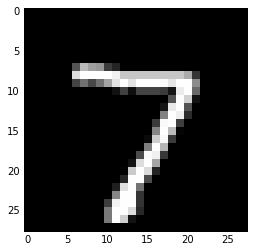
\includegraphics[width=\linewidth]{../images/image-1.png}
  \caption{Image 1}
  \label{fig:image-1}
\end{figure}

Figure \ref{fig:hl1} shows the image as it passes through the first
hidden layer of the network. We can see the image is beginning to
distort, but we can still determine what the image is.

\begin{figure}
  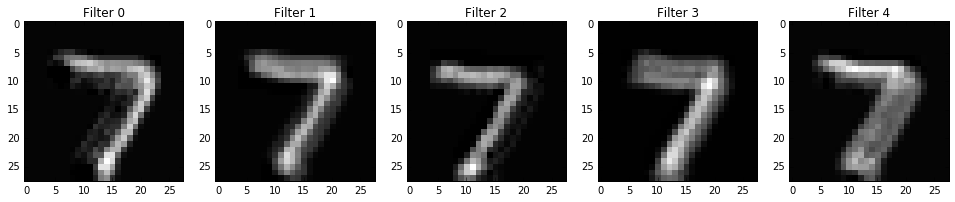
\includegraphics[width=\linewidth]{../images/hl1.png}
  \caption{First Hidden Layer}
  \label{fig:hl1}
\end{figure}

Figure \ref{fig:hl2} shows the image as it passes through the second
hidden layer of the network. The image is now distorted even more as it
works it way through the network.\\

\begin{figure}
  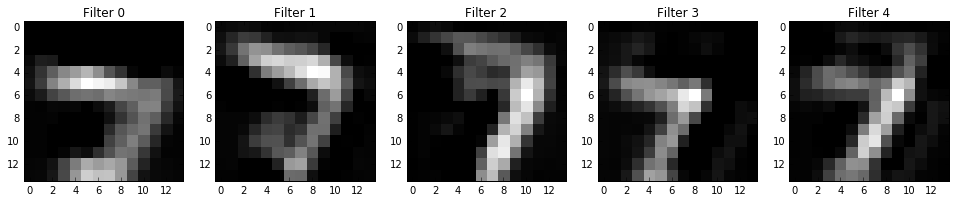
\includegraphics[width=\linewidth]{../images/hl2.png}
  \caption{Second Hidden Layer}
  \label{fig:hl2}
\end{figure}

Finally, Figure \ref{fig:hl3} shows the image as it passes through the
third hidden layer of the network. At this point the network is passing
the image into and out of 20 filters in order to capture all the data
necessary for training. This demonstrates the ``deep'' context of deep
learning.\\

\begin{figure}
  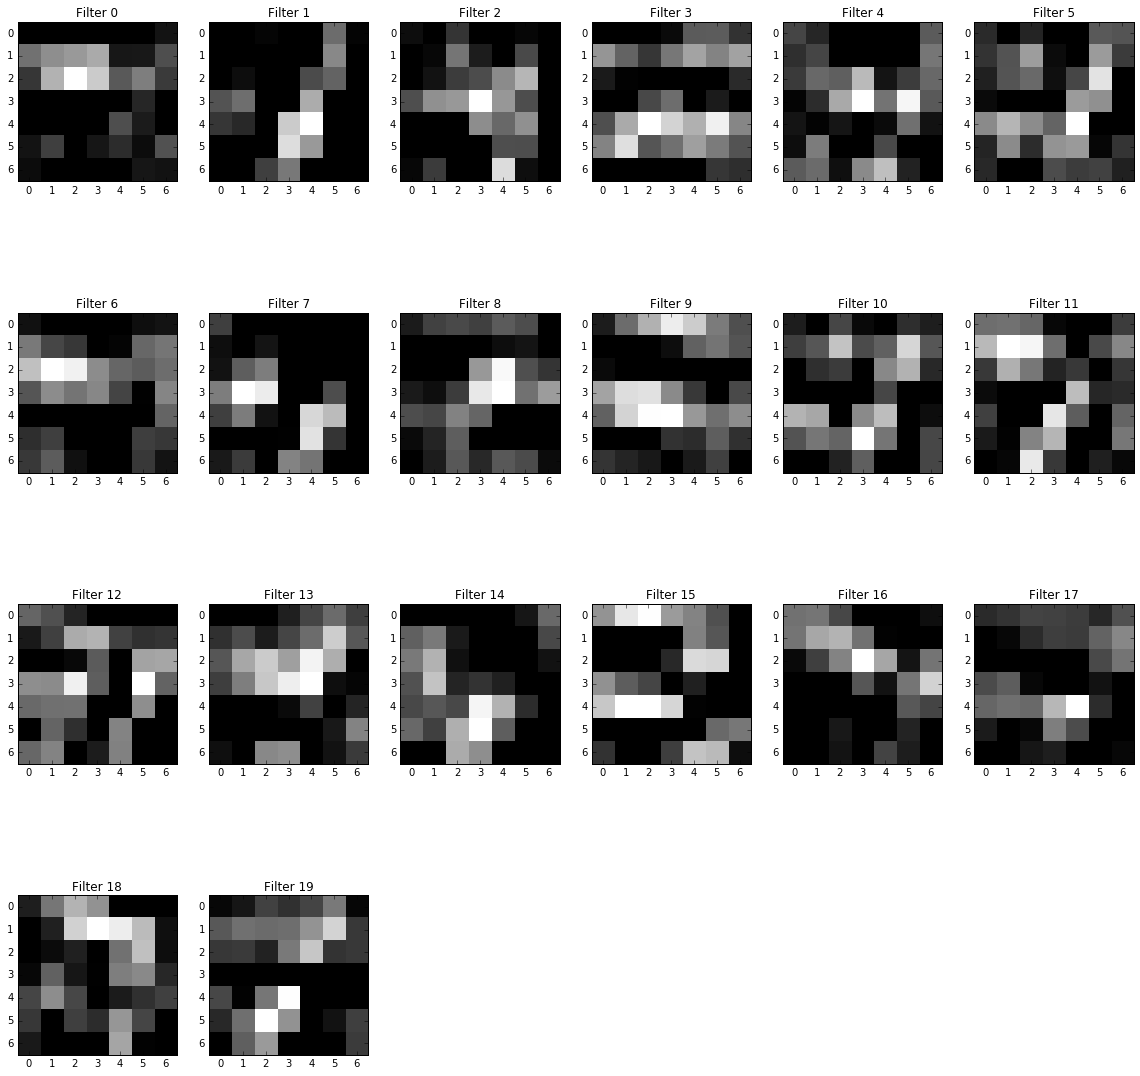
\includegraphics[width=\linewidth]{../images/hl3.png}
  \caption{Third Hidden Layer}
  \label{fig:hl3}
\end{figure}

As stated in the previous subsection, the results are split into four
separate scenarios to measure both the number of steps to convergence
and the accuracy at convergence. Table \ref{table:accr} below summarizes
the number of steps, max accuracy, and step number at which max accuracy
was obtained.

The first iteration of \(1000\) steps has a high accuracy rate at
\(900\) steps, with a max accuracy calculation of \(0.984\). The next
iteration was at \(2500\), with a max accuracy calculation of \(0.988\)
at \(2200\). The third iteration consisted of \(5000\) steps, a max
accuracy calculation of \(0.9918\) at 4800 steps, and finally, the last
iteration consisted of \(10000\) steps, and obtained a max accuracy
calculation of \(0.9928\) at \(8400\) steps.

\begin{table}[h]
    \caption{Steps and Max Accuracy}
    \centering
        \begin{tabular}{c c c}
            \hline \hline
            Steps & Max Step\# & Accuracy \\ [1ex]
            \hline
            1000  & 900  & 0.984 \\
            2500  & 2200 & 0.9888 \\
            5000  & 4800 & 0.9918 \\
            10000 & 8400 & 0.9928 \\  [1ex]
            \hline
        \end{tabular}
    \label{table:accr}
\end{table}

The main observation of the results is that as the model steps
increased, and stepped through the data, the model tended to learn at a
slower rate, but produced results with greater accuracy. That said,
given a larger machine, faster processor, and continued training on the
the dataset as a whole, I am confident the convolutional neural network
would converge to near 100\%. As seen in Table \ref{table:accr}, the
number of steps increased, for each interation, in order to reach max
accuracy. This makes sense, given the model has more steps to process,
and essentially more time to learn.

\section{V. Conclusion and Future
Work}\label{v.-conclusion-and-future-work}

Image processing with convolutional neural networks was a ground
breaking rediscovery, applying long forgotten algorithms and theories to
a new and interesting problem. The speed and accuracy of convolutional
neural network makes the algorithm a prime candidate to apply in the
fields of cybersecurity, threat detection, facial recognition, as well
as physics and quantum computing and engineering. A practitioner with a
laptop and an internet connection can calculate on large datasets,
without having to consider server time and availability.

I believe we are only scratching the surface of what deep learning and
convolutional neural networks can do. As more and more data becomes
available, and with more research and experimentation, advancing deep
learning will become easier and more valuable for everyday life.

\section{Acknowledgment}\label{acknowledgment}

I would like to thank the students in Old Dominion University's MSIM 607
machine learning class. The dialogue and discussions aided in my
comprehension of the information; Melissa Rich for assisting with
proofreading this paper; Dr.~Li for his patience and understanding; my
staff for offering ideas to improve and optimize the code, and my family
for letting me write in peace and quiet.

\newpage

\section*{References}\label{references}
\addcontentsline{toc}{section}{References}

\hypertarget{refs}{}
\hypertarget{ref-h2o}{}
Ambati, S., and C. Click. n.d. ``H2O Documentation.'' Available at
\url{https://www.h2o.ai} (2018/04/28).

\hypertarget{ref-py3}{}
Anaconda. n.d. ``Anaconda Distribution 5.'' Available at
\url{https://docs.anaconda.com/} (2018/04/28).

\hypertarget{ref-bishop2006}{}
Bishop, C M. 2006. \emph{Pattern Recognition and Machine Learning}.
Cambridge CB3 0FB, U.K.: Springer.
\url{https://www.springer.com/us/book/9780387310732}.

\hypertarget{ref-sgd2010}{}
Bottou, L. 2010. ``Large-Scale Machine Learning with Stochastic Gradient
Descent.'' In \emph{Proceedings of 19th International Conference
Computer Statistics}, 177--86. Princeton, NJ: Springer.

\hypertarget{ref-dwivedi2018}{}
Dwivedi, P. 2018. ``Handwriting Recognition Using Tensorflow and
Keras.'' \emph{Towards Data Science}. January.
\url{https://towardsdatascience.com/handwriting-recognition-using-tensorflow-and-keras-819b36148fe5}.

\hypertarget{ref-goodfellow2016}{}
Goodfellow, I, Y Bengio, and A Courville. 2016. \emph{Deep Learning}.
1st ed. Cambridge, MA: MIT Press. \url{http://www.deeplearningbook.org}.

\hypertarget{ref-keras}{}
keras-team. n.d. ``Keras Documentation.'' Available at
\url{https://keras.io} (2018/04/28).

\hypertarget{ref-lecun1998}{}
LeCun, Y, L Bottou, Y Bengio, and P Haffner. 1998. ``Gradient-Based
Learning Applied to Document Recognition.'' In \emph{Proceedings of the
IEEE}, 86:2278--2324. 11.
\url{http://yann.lecun.com/exdb/publis/pdf/cox-98.pdf}.

\hypertarget{ref-sgd2013}{}
Sutskever, I, J Martens, G Dahl, and G Hinton. 2013. ``On the Importance
of Initialization and Momentum in Deep Learning.'' In \emph{Proceedings
of the 30th International Conference on Machine Learning}, 1139--47.
ICML.

\hypertarget{ref-tfr18}{}
TensorFlow. n.d. ``API R1.8.'' Available at
\url{https://www.tensorflow.org/api_docs/python/} (2018/04/28).

\end{document}


